\chapter{Vandermonde-Matrizen mit Stützstellen auf dem Einheitskreis}

Wie das vorherige Kapitel zeigt, sind Vandermonde-Matrizen mit reellen
Stützstellen schlecht konditioniert und werden daher hauptsächlich für
theoretische Betrachtungen verwendet.

Anders verhält es sich, wenn man Knoten in der komplexen Ebene zulässt.
Wählt man als Stützstellen die $n$-ten Einheitswurzeln, so erreicht die
Vandermonde-Matrix sogar die perfekte Kondition $1$ bezüglich der Spektralnorm.

In diesem Abschnitt untersuchen wir Vandermonde-Matrizen mit Knoten auf dem
komplexen Einheitskreis, die jedoch von dem perfekten Fall der $n$-ten
Einheitswurzeln abweichen.
Für diese speziellen Konfigurationen leiten wir explizite Formeln zur
Berechnung der Kondition bezüglich der Zeilensummennorm und der Frobeniusnorm
her.

\section{Vandermonde-Matrizen zu den \boldmath $n$-ten Einheitswurzeln}

\begin{lemma}
    \label{lemma:frobenius_norm_vandermonde_unit_circle}
    Für Knoten auf dem Einheitskreis
    $z = \left(e^{i \varphi_0}, \dots, e^{i \varphi_{n-1}} \right) \in \C$
    mit $\varphi_j \in \R$ für $j = 0, \dots, n-1$ gilt
    \begin{equation}
        \norm{\Vand{z}}_F = n.
    \end{equation}
\end{lemma}
\begin{proof}
    Es gilt
    \[
        \norm{\Vand{z}}_F^2
        = \sum_{k=0}^{n-1} \sum_{j=0}^{n-1} \abs{ \left(e^{i \varphi_j}\right)^k }^2
        = \sum_{k=0}^{n-1} \sum_{j=0}^{n-1} 1
        = n^2.
    \]
\end{proof}


\begin{lemma}
    Sei $n \in \N$ und $z = (z_0, \dots, z_{n-1}) \in \Cn$ der Vektor der
    $n$-ten Einheitswurzeln, also $z_j = e^{\frac{2 \pi i j}{n}}$ für
    $j = 0, \dots, n-1$.
    Dann gilt für die Kondition bzgl. der Frobeniusnorm
    \[
        \cond[F]{\Vand{z}} = n.
    \]
\end{lemma}
\begin{proof}
    Wir setzen $W = (w_{jr})_{j,r=0}^{n-1} \in \C^{n\times n}$ mit
    $w_{jr} \defeq \frac{1}{n} e^{- \frac{2 \pi i j r}{n}}$
    und zeigen $V^{-1} = W$.
    Seien dazu $a_{kr} \in \C$ die Elemente des Matrixproduktes
    $A = V W \in \C^{n\times n}$.
    Dann gilt für $k, r = 0, \dots, n-1$
    \[
        \begin{split}
            a_{kr}
            &= \sum_{j=0}^{n-1} v_{kj} w_{jr}
            = \sum_{j=0}^{n-1} \frac{1}{n} \exp \left( \frac{2 \pi i k j}{n} \right) \exp \left( -\frac{2 \pi i j r}{n} \right)\\
            &= \frac{1}{n} \sum_{j=0}^{n-1} \exp \left( \frac{2 \pi i j (k - r)}{n} \right)
            = \frac{1}{n} \sum_{j=0}^{n-1} \left( \exp \left( \frac{2 \pi i (k - r)}{n} \right) \right)^j\\
            &= \frac{1}{n} \cdot \left\{
                \begin{array}{ll}
                    n, \text{ falls } k-r \equiv 0 \mod n\\
                    0, \text{ falls } k-r \not\equiv 0 \mod n
                \end{array}
              \right.\\
            &= \left\{
                \begin{array}{ll}
                    1, \text{ falls } k = r \\
                    0, \text{ falls } k \neq r .
                \end{array}
              \right.
        \end{split}
    \]
    Damit ist $V^{-1} = W$ gezeigt.
    Nach Lemma \ref{lemma:frobenius_norm_vandermonde_unit_circle} gilt $\norm{V}_F = n$
    und damit $\norm{V^{-1}}_F = \norm{W}_F = \frac{1}{n} \norm{\overline V}_F = 1$,
    was die Behauptung zeigt.
\end{proof}


\section{Invarianz der Kondition unter Rotation der Knoten}

Im Folgenden zeigen wir, dass sich die Kondition einer Vandermonde-Matrix
bezüglich der Zeilensummennorm und aller unitär invarianten Normen weder unter
Rotation noch unter Spiegelung der Knoten verändert.

%TODO: Was bringt das?

\begin{lemma}
    \label{lemma:vandermonde_rotation_invariance}
    Die Kondition der Vandermonde-Matrix bezüglich der Zeilensummennorm ist
    invariant unter Multiplikation der Knoten mit einer komplexen Zahl
    $\alpha = e^{i\varphi} \in \C$ mit $\varphi \in \R$.
\end{lemma}
\begin{proof}
    Sei $z = (z_0, \dots, z_{n-1}) \in \Cn$.
    Wegen $\abs{e^{i\varphi}} = 1$ für alle $\varphi \in \R$ gilt
    \[
        \begin{split}
            \norm{\Vand{\alpha z}}_\infty
            &= \max_{k=0, \dots, n-1} \sum_{j=0}^{n-1} \abs{\left(e^{i\varphi} z_j\right)^k}
            = \max_{k=0, \dots, n-1} \sum_{j=0}^{n-1} \abs{e^{ik\varphi}} \abs{z_j^k}\\
            &= \max_{k=0, \dots, n-1} \sum_{j=0}^{n-1} \abs{z_j^k}
            = \norm{\Vand{z}}_\infty.
        \end{split}
    \]

    \noindent Für die Zeilensummennorm der inversen Vandermonde-Matrix erinnern
    wir uns an Gleichung
    (\ref{eq:inverse_vandermonde_const_multiplication})
    aus Lemma \ref{lemma:vandermonde_const_multiplication}:
        $\Vand{\alpha z}^{-1}
        = \Vand{z}^{-1} \cdot \diag{\alpha^0, \alpha^{-1}, \dots, \alpha^{-n+1}}.$
    Damit ist sofort ersichtlich, dass
    \[
        \begin{split}
            \norm{\Vand{\alpha z}^{-1}}_\infty
            &= \max_{j=0, \dots, n-1} \sum_{r=0}^{n-1} \abs{u_{jr}} \abs{\alpha^{-r}}\\
            &= \max_{j=0, \dots, n-1} \sum_{r=0}^{n-1} \abs{u_{jr}}
            = \norm{\Vand{\alpha}^{-1}}_\infty.
        \end{split}
    \]

    \noindent Wie behauptet folgt insgesamt
    \[
        \begin{split}
            \cond[\infty]{\Vand{\alpha z}}
            &= \norm{\Vand{\alpha z}}_\infty \norm{\Vand{\alpha z}^{-1}}_\infty\\
            &= \norm{\Vand{z}}_\infty \norm{\Vand{z}^{-1}}_\infty
            = \cond[\infty]{\Vand{z}}.
        \end{split}
    \]
\end{proof}

\begin{lemma}
    Sei $\emptynorm$ eine Matrix-Norm, die invariant unter Multiplikation mit unitären
    Matrizen ist, d.h. für jede Matrix $A \in \C^{n\times n}$ und jede
    unitäre Matrix $U \in \C^{n\times n}$ gilt $\norm{UA} = \norm{AU} = \norm{A}$.
    Weiter seien ein Vektor $z = (z_0, \dots, z_{n-1}) \in \Cn$ und eine
    komplexe Zahl $\alpha \in \C$ mit Betrag $\abs{\alpha} = 1$ gegeben.
    Dann gilt für die Kondition bezüglich der Norm $\emptynorm$
    \[
        \cond{\Vand{\alpha z}} = \cond{\Vand{z}},
    \]
    d.h. die Kondition der Vandermonde-Matrix ist in diesem Fall invariant
    unter Multiplikation der Knoten mit einer komplexen Zahl $\alpha$ vom
    Betrag $\abs{\alpha} = 1$.
\end{lemma}
\begin{proof}
    Nach Lemma \ref{lemma:vandermonde_const_multiplication} gelten
    \[
        \norm{ \Vand{\alpha z} }
        \overset{(\ref{eq:vandermonde_const_multiplication})}{=}
            \norm{\diag{\alpha^0, \dots, \alpha^{n-1}} \cdot \Vand{z}}
    \]
    und
    \[
        \norm{ \Vand{\alpha z}^{-1} }
        \overset{(\ref{eq:inverse_vandermonde_const_multiplication})}{=}
            \norm{\Vand{z}^{-1} \cdot \diag{\alpha^0, \alpha^{-1}, \dots, \alpha^{-n+1}}}.
    \]
    Mit $e^{i \varphi} \defeq \alpha$ für ein $\varphi \in \R$ stellen wir
    leicht fest, dass
    $\diag{\alpha^0, \alpha^1, \dots, \alpha^{n-1}}$ eine unitäre Matrix ist:
    \[
        \begin{split}
            \diag{\alpha^0, \alpha^1, \dots, \alpha^{n-1}}^H
            &= \diag{1, e^{i \varphi}, \dots, e^{(n-1) i \varphi}}^H\\
            &= \diag{1, e^{-i \varphi}, \dots, e^{-(n-1) i \varphi}}\\
            &= \diag{1, e^{i \varphi}, \dots, e^{(n-1) i \varphi}}^{-1}\\
            &= \diag{\alpha^0, \alpha^1, \dots, \alpha^{n-1}}^{-1},
        \end{split}
    \]
    wobei $A^H$ die adjungierte Matrix von $A$ bezeichne.
    \noindent Insgesamt folgt
    \[
        \begin{split}
            \cond{\Vand{\alpha z}}
            &= \norm{\Vand{\alpha z}} \norm{\Vand{\alpha z}^{-1}}\\
            &= \norm{\diag{\alpha^0, \dots, \alpha^{n-1}} \cdot \Vand{z}} \norm{\Vand{z}^{-1} \cdot \diag{\alpha^0, \alpha^{-1}, \dots, \alpha^{-n+1}}}\\
            &= \norm{\Vand{z}} \norm{\Vand{z}^{-1}}
            = \cond{\Vand{z}}.
        \end{split}
    \]
\end{proof}

% SECTION:OUTLIER
\section{Vandermonde-Matrizen aus \boldmath{$(n\!-\!1)$} Einheitswurzeln und einem Ausreißer}

Im Folgenden untersuchen wir die Kondition einer Vandermonde-Matrix zu den
Knoten der $n$-ten Einheitswurzeln, wobei einer der Knoten von seiner
ursprünglichen Position um einen Winkel $\delta \in \left[0,\frac{2
\pi}{n}\right)$ auf dem Einheitskreis ausgelenkt wird.
Wie bereits in Lemma \ref{lemma:vandermonde_rotation_invariance} gezeigt,
ändern weder Drehungen noch Spiegelungen der Knoten die Kondition der
Vandermonde-Matrix.
Daher können wir ohne das Problem zu beschränken, stets den Knoten auslenken,
welcher der $n$-ten Einheitswurzel $1$ zugeordnet ist.

Wir betrachten also den Vektor $z(\delta) = (z_0(\delta), z_1, \dots, z_{n-1}) \in \C^n$ mit
$z_0(\delta) = e^{2 \pi i \delta / n}$
und
$z_j = e^{2 \pi i j / n}$ für $j = 1, \dots, n-1$
sowie die dazu gehörende Vandermonde-Matrix, die wir in diesem Abschnitt
mit $\Vand{\delta} \defeq \Vand{z(\delta)}$ bezeichnen.
Häufig werden wir auf die explizite Angabe der Abhängigkeit von $\delta$
verzichten, und beispielsweise nur kurz $z_0$ anstelle von $z_0(\delta)$
schreiben.

\subsection{Kondition bezüglich der Zeilensummennorm}

Vandermonde-Matrizen mit Stützstellen innerhalb des komplexen Einheitskreises
haben die Zeilensummennorm $n$, wie bereits in
\lemmaref{infty_norm_vandermonde_unit_roots} gezeigt wurde.
Dies trifft offensichtlich auch in unserem Fall zu, so dass wir für die
Berechnung der Kondition nur noch die Zeilensummennorm der inversen
Vandermonde-Matrix $\Vand{\delta}^{-1}$ ermitteln müssen.

\begin{lemma}
    \label{lemma:inverse_outlier_vandermonde_first_row_abs_sum}
    Sei $z(\delta) = (z_0(\delta), \dots, z_{n-1}) \in \C^n$ mit
    $z_0(\delta) = e^{2 \pi i \delta / n}$
    und
    $z_j = e^{2 \pi i j / n}$ für $j = 1, \dots, n-1$.
    Weiter seien $u_{jr} \in \C$ für $j,r = 0,\dots,n-1$ die Elemente der
    inversen Vandermonde-Matrix $\Vand{z(\delta)}^{-1}$.
    Dann gilt
    \[
        \sum_{r=0}^{n-1} \abs{ u_{0r} }
        = n \cdot \prod_{k=1}^{n-1} \abs{z_0 - z_k}^{-1}
        = n \cdot \prod_{j=1}^{n-1} \frac{1}{2 \cdot \sin \left(\frac{\pi (j - \delta)}{n} \right)}.
    \]
\end{lemma}

\begin{proof}
    Nach Gleichung (\ref{eq:explicit_inverse_vandermonde}) gilt
    \[
        u_{0r} = (-1)^{n-1-r} \cdot \Pi_0 \cdot \sigma_{n-1-r}^{0}(z_1, \dots, z_{n-1})
    \]
    mit
    \[
        \Pi_0 = \prod_{k=1}^{n-1} \abs{ z_0 - z_k }^{-1}.
    \]

    \noindent Sei $k \in \{1, \dots, n-1\}$ und $\varphi \defeq \frac{\pi (k - \delta)}{n}$.
    Dann gilt
    \[
        \begin{split}
            \abs{z_0 - z_k}^2
            &= (z_0 - z_k) (\conj{z}_0 - \conj{z}_k)
            = \abs{z_0}^2 + \abs{z_k}^2 - z_0\conj{z}_k - z_k\conj{z}_0\\
            &= 2 - (e^{2 \varphi i} + e^{-2 \varphi i})
            = 2 - ((e^{\varphi i})^2 + (e^{-\varphi i})^2)\\
            &= 2 - ( (e^{\varphi i} - e^{-\varphi i})^2 + 2 e^{(\varphi - \varphi) i})
            = (e^{\varphi i} - e^{-\varphi i})^2\\
            &= 4 \cdot \sin^2 (\varphi)
            = 4 \cdot \sin^2 \left( \frac{\pi (k-\delta)}{n} \right),
        \end{split}
    \]
    also
    \begin{equation}
        \label{eq:pi_0}
        \Pi_0
        = \prod_{\substack{k = 1}}^{n-1} \abs{ z_0 - z_k }^{-1}
        = \prod_{\substack{k = 1}}^{n-1} \frac{1}{2 \cdot \sin \left( \frac{\pi (k-\delta)}{n} \right)}.
    \end{equation}

    \noindent Zusammen mit der Aussage des Korollars
    \ref{corollary:outlier_sigma_zero_row_sum} folgt nun die Behauptung:
    \[
        \begin{split}
            \sum_{r=0}^{n-1} \abs{ u_{0r} }
            &= \sum_{r=0}^{n-1} \abs{ (-1)^{n-1-r} \cdot \Pi_0 \cdot \sigma_{n-1-r}(z_1, \dots, z_{n-1}) }\\
            &= \left( \sum_{r=0}^{n-1} \abs{ \sigma_{n-1-r}(z_1, \dots, z_{n-1}) } \right) \cdot \abs{\Pi_0}\\
            &\overset{(\ref{eq:outlier_sigma_zero_row_sum})}{=}
                n \cdot \prod_{j=1}^{n-1} \frac{1}{2 \cdot \sin \left(\frac{\pi (j - \delta)}{n} \right)}.
        \end{split}
    \]
\end{proof}

Der Beweis der folgenden Vermutung kann im Rahmen dieser Arbeit nicht
erbracht werden. Numerische Untersuchungen konnten die Aussage jedoch nicht
widerlegen.

\begin{assumption}
    Es gilt
    \begin{equation}
        \cond[\infty]{ \Vand{\delta} }
        = n^2 \prod_{j=1}^{n-1} \abs{ z_0(\delta) - z_j }^{-1}
        = n^2 \prod_{j=1}^{n-1} \frac{1}{2 \cdot \sin \left(\frac{\pi (j - \delta)}{n} \right)}.
    \end{equation}
\end{assumption}

\begin{remark}
    Zum Beweis der Vermutung muss gezeigt werden, dass
    \[
        \norm{\Vand{\delta}^{-1}}_\infty
        = n \cdot \prod_{j=1}^{n-1} \frac{1}{2 \cdot \sin \left(\frac{\pi (j - \delta)}{n} \right)}.
    \]
    gilt.
    Bezeichnen wir erneut mit $u_{jr}$ für $j,r = 0, \dots, n-1$ die Elemente von $\Vand{\delta}^{-1}$,
    so bleibt zu zeigen, dass für $j = 1, \dots, n-1$
    \[
        \sum_{r=0}^{n-1} \abs{u_{jr}} \leq \sum_{r=0}^{n-1} \abs{u_{0r}}
    \]
    gilt.
    Lemma \ref{lemma:inverse_outlier_vandermonde_first_row_abs_sum} liefert dann die Behauptung.

    \noindent Der Ansatz, die beiden Faktoren $\Pi_j$ und
    $\sum_{r=0}^{n-1} \abs{\sigma_r^j}$ einzeln abzuschätzen,
    d.h. die Ungleichungen
    \[
        \Pi_j \leq \Pi_0
    \]
    und
    \[
        \sum_{r=0}^{n-1} \abs{\sigma_r^j} \leq \sum_{r=0}^{n-1} \abs{\sigma_r^0}
    \]
    für alle $ j=1, \dots, n-1$ zu beweisen, muss im Allgemeinen scheitern, wie
    die Figuren \ref{fig:pi_j} und \ref{fig:sigma_row_sum} für den Fall $n=5$ zeigen.
    Die schwarzen Graphen, die den Fall $j=0$ darstellen, nehmen dort niemals
    den Maximalwert unter allen Graphen von $j=0, \dots, n-1$ an.
    Die Figur \ref{fig:row_j} legt jedoch nahe, dass die Behauptung des
    Satzes tatsächlich wahr ist, denn der Graph des Produktes ist stets für
    $j=0$ maximal.

    \noindent Der Beweis kann also nur erbracht werden, indem das gesamte Produkt
    abgeschätzt wird:
    \[
        \Pi_j \sum_{r=0}^{n-1} \abs{\sigma_r^j} \leq \Pi_0 \sum_{r=0}^{n-1} \abs{\sigma_r^0} \text{ für } j=1, \dots, n-1.
    \]
\end{remark}

%\begin{figure}[htb]
%    \centering
%    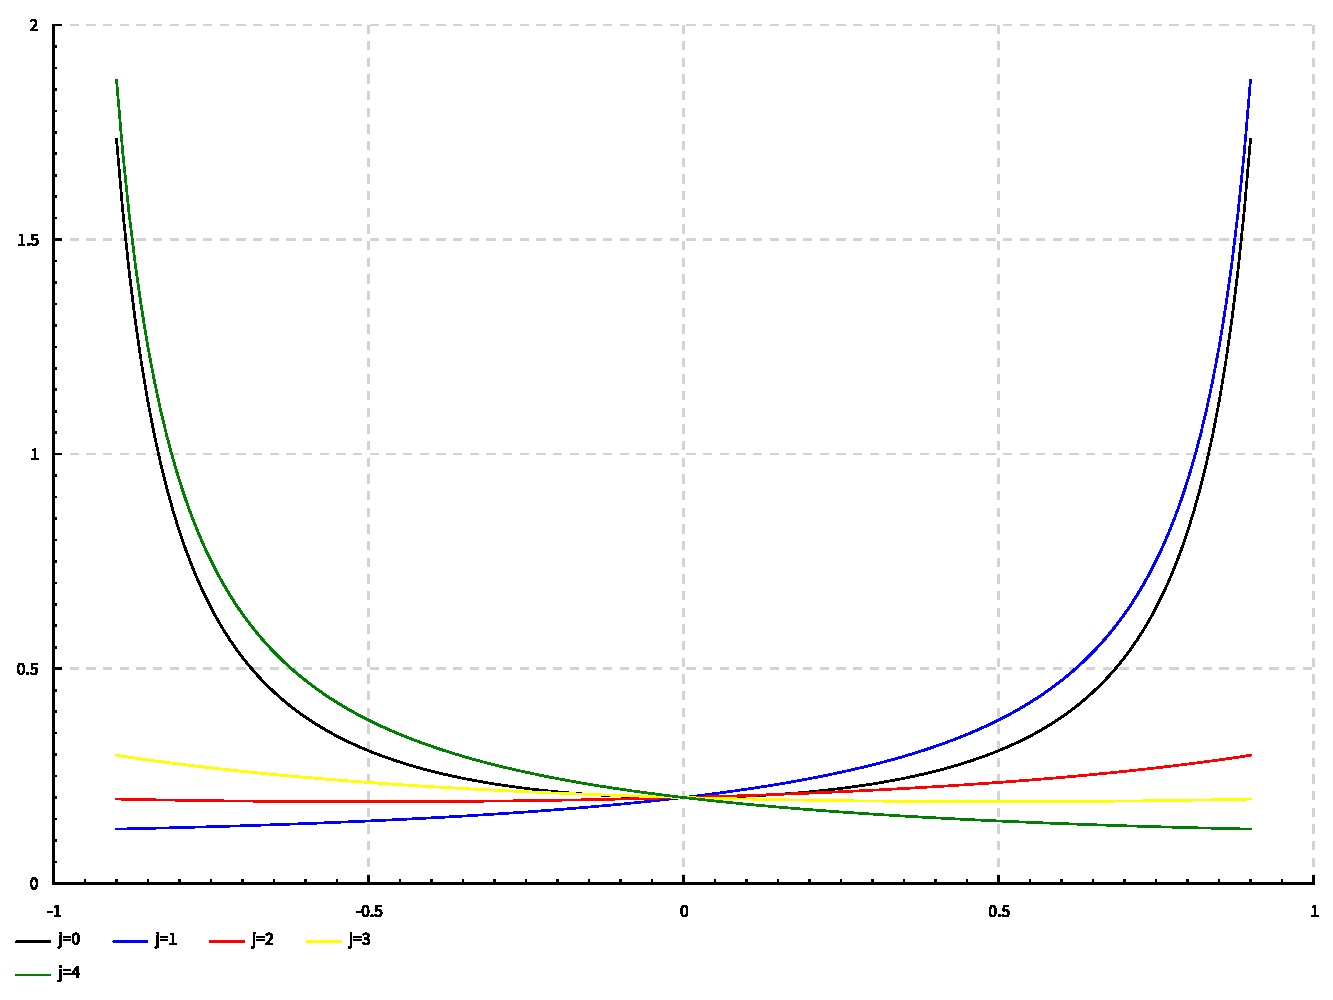
\includegraphics[width=350pt]{images/pi_j}
%    \caption{$ f_j(\delta) = \Pi_j(\delta) $}
%    \label{fig:pi_j}
%\end{figure}
%
%\begin{figure}[htb]
%    \centering
%    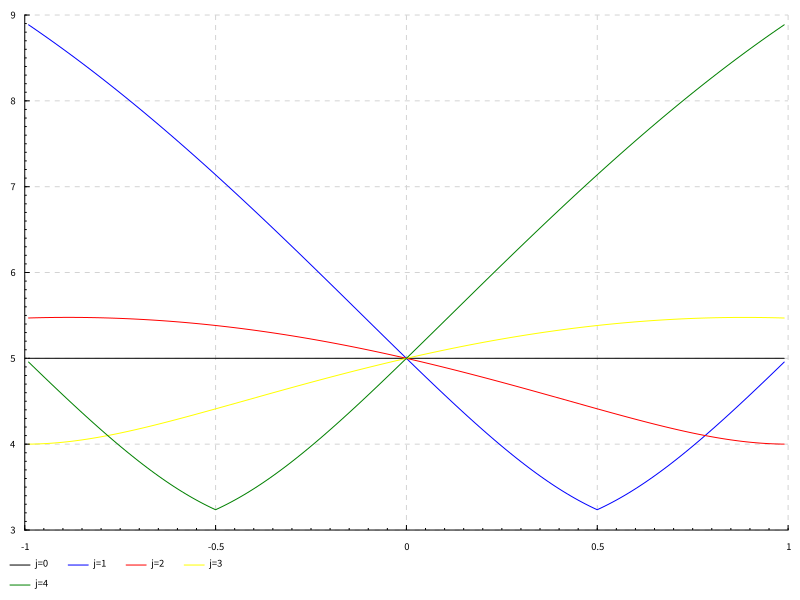
\includegraphics[width=350pt]{images/sigma_row_sum}
%    \caption{$ g_j(\delta) = \sum_{r=0}^{n-1} \abs{ \sigma_r^j(z(\delta)) } $}
%    \label{fig:sigma_row_sum}
%\end{figure}
%
%\begin{figure}[htb]
%    \centering
%    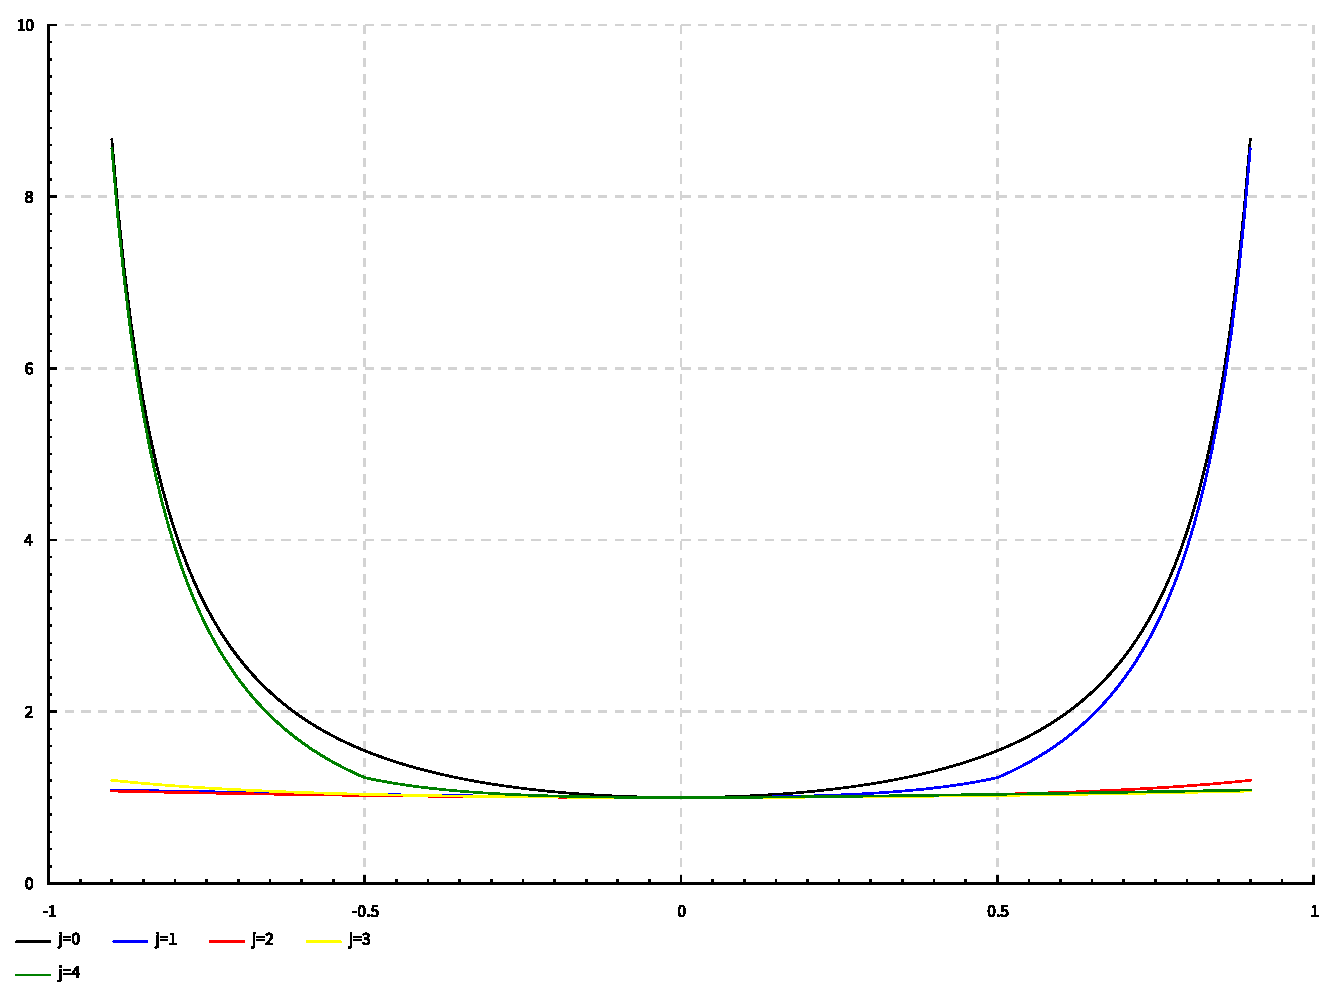
\includegraphics[width=350pt]{images/row_j}
%    \caption{$ h_j(\delta) = \sum_{r=0}^{n-1} \abs{ u_{jr}(\delta) } $}
%    \label{fig:row_j}
%\end{figure}

\subsection{Kondition bezüglich der Frobeniusnorm}
% FIXME: Next paragraph is crap.
Wir wollen nun eine explizite Formel für die Kondition der Vandermonde-Matrix
$\Vand{\delta}$ bezüglich der Frobeniusnorm beweisen.
Dazu sei an die Definition der Frobeniusnorm (\ref{eq:frobenius_norm}) erinnert.
Bereits in Lemma \ref{lemma:frobenius_norm_vandermonde_unit_circle} wurde
gezeigt, dass die Norm einer Vandermonde-Matrix mit $n$ Knoten auf dem
Einheitskreis $n$ beträgt.
Schwierigkeiten kann also nur die Norm der inversen Vandermonde-Matrix
bereiten.  Wir betrachten im Folgenden die zwei Fälle $j=0$ und
$j \in \{1, \dots, n-1\}$ gesondert.

\begin{lemma}
    \label{lemma:inverse_outlier_zero_row_quadratic_sum}
    Bezeichnen wir mit $u_{jr} \in \C$ für $j, r = 0, \dots, n-1$ die Elemente
    der inversen Vandermonde-Matrix $V(\delta)^{-1}$, so gilt
    \[
        \sum_{r=0}^{n-1} \abs{u_{0r}}^2
        = n \cdot \prod_{k=1}^{n-1} \frac{1}{4 \cdot \sin^2 \left( \pi \frac{k-\delta}{n} \right)}.
    \]
\end{lemma}
\begin{proof}
    % TODO: Hier fehlt noch der Hinweis auf pi_0, die Formel erscheint aus dem
    % Nichts.
    Mit Lemma \ref{lemma:outlier_sigma_zero} und Gleichung (\ref{eq:pi_0}) aus
    dem Beiweis von \lemmaref{inverse_outlier_vandermonde_first_row_abs_sum}
    erhalten wir
    \[
        \begin{split}
            \sum_{r=0}^{n-1} \abs{u_{0r}}^2
            &= \sum_{r=0}^{n-1} \abs{\Pi_0}^2 \abs{\sigma_{n-1-r}^{0}(z_1, \dots, z_{n-1})}^2\\
            &\overset{(\ref{eq:outlier_sigma_zero})}=
                \abs{\Pi_0}^2 \sum_{r=0}^{n-1} 1^2
            = n \cdot \abs{\Pi_0}^2\\
            &\overset{(\ref{eq:pi_0})}=
                n \cdot \prod_{k=1}^{n-1} \frac{1}{4 \cdot \sin^2 \left( \pi \frac{k-\delta}{n} \right)}.
        \end{split}
    \]
\end{proof}

\noindent Als Vorbereitung für den Fall $j \in \{1, \dots, n-1\}$ benötigen wir noch zwei
Hilfslemmata.
\begin{lemma}
    \label{lemma:uptau_j}
    Sei $\w_n \defeq e^{\frac{2 \pi i}{n}}$.
    Definiere $\uptau_j \in \C$ für $j=0, \dots, n-1$ durch
    \[
        \uptau_j \defeq \prod_{\substack{k=0\\k\neq j}}^{n-1} \left( \w_n^j - \w_n^k\right).
    \]
    Dann gilt $\abs{\uptau_j} = n$ für alle $j = 0, \dots, n-1$.
\end{lemma}
\begin{proof}
    Wir zeigen $\abs{\uptau_j} = \abs{\uptau_0}$ für alle $j = 1, \dots, n-1$ und
    $\uptau_0 = n$.
    Es gilt
    \[
        \begin{split}
            \abs{\uptau_j}
            &= \abs{\uptau_j \cdot \w_n^{-j}}
            = \prod_{\substack{k=0\\ k\neq j}}^{n-1} \abs{\w_n^0 - \w_n^{k-j} }\\
            &\overset{k' = k-j}{=}
            \prod_{\substack{k'=-j\\ k\neq 0}}^{n-1-j} \abs{1 - \wn^{k'}}
            = \prod_{\substack{k'=0\\ k\neq 0}}^{n-1} \abs{1 - \wn^{k'}}
            = \abs{\uptau_0},
        \end{split}
    \]
    wobei wir im letzten Schritt nur die Reihenfolge der Faktoren verändern und
    die $2\pi$-Periodizität von $e^{i \varphi}$ ausnutzen.

    \noindent Mit $p(z) \defeq \prod_{k=1}^{n-1} (z - \wn^k)$ können wir $\uptau_0 = p(1)$
    schreiben.

    Bereits im Beweis von \lemmaref{outlier_sigma_zero} haben wir gesehen, dass
    \[
        p(z) = \prod_{k=1}^{n-1} (z-\w_n^k) = \sum_{k=0}^{n-1} z^k
    \]
    gilt.
    Damit folgt sofort
    \[
        \uptau_0 = p(1) = \sum_{k=0}^{n-1} 1^k = n.
    \]
\end{proof}

\begin{lemma}
    \label{lemma:sum_shifted_unit_roots}
    Für $j \in \{1, \dots, n-1\}$ gilt
    \[
        \sum_{r=0}^{n-1} \cos \left( \frac{2 \pi j r}{n} - \varphi \right) = 0.
    \]
\end{lemma}
\begin{proof}
    Mit $p(z) \defeq \sum_{k=0}^{n-1} z^n = \prod_{j=1}^{n-1} (z - \wn^j)$ gilt
    \[
        \begin{split}
            \sum_{r=0}^{n-1} \cos \left( \frac{2 \pi j r}{n} - \varphi \right)
            &= \sum_{r=0}^{n-1} \Re\left( e^{\frac{2 \pi i j r}{n} - i \varphi} \right)
            = \Re \left( \sum_{r=0}^{n-1} e^{\frac{2 \pi i j r}{n} - i \varphi} \right)\\
            &= \Re \left( e^{-i \varphi}\sum_{r=0}^{n-1} \left( \wn^j \right)^r \right)
            = \Re \left( e^{-i \varphi} p\left( \wn^j \right) \right)
            = 0,
        \end{split}
    \]
    wobei $\Re(z)$ den Realteil von $z$ bezeichnet.
\end{proof}

\begin{lemma}
    \label{lemma:inverse_outlier_nonzero_row_quadratic_sum}
    Sei $z(\delta) = (z_0(\delta), z_1, \dots, z_{n-1}) \in \Cn$ wie zuvor.
    Erneut bezeichnen wir mit $u_{jr}$ die Elemente der inversen
    Vandermonde-Matrix $\Vand{\delta}^{-1}$.
    Dann gilt für ${j = 1, \dots, n-1}$
    \begin{equation}
        \sum_{r=0}^{n-1} \abs{u_{jr}}^2
        = \frac{\rho(\delta)^2 + 1}{n}
    \end{equation}
    mit
    \[
        \rho(\delta) \defeq \frac{\sin \left( \pi \frac{\delta}{n} \right)}{\sin \left( \pi \frac{j - \delta}{n} \right)}.
    \]
\end{lemma}
\begin{proof}
    In diesem Beweis werden wir der Übersicht wegen meist auf die explizite
    Erwähnung der Abhängigkeit von $\delta$ verzichten und nur kurz
    $z_0 = z_0(\delta)$ schreiben.

    \noindent Sei $j \in \{1, \dots, n-1\}$ fixiert.
    Wir erinnern uns zunächst daran, dass mit Lemma
    \ref{lemma:elementary_symmetric_polynomials_const_multiplication}
    für ${r = 0, \dots, n-1}$
    \[
        \abs{ \sigma_r^j (z)}
        = \abs{(-1)^r \sigma_r^j (-z) }
        = \abs{\sigma_r^j (-z) }
    \]
    gilt.
    Weiterhin ist nach Definition $\sigma_r^j (-z)$ der $n\!-\!j\!-\!1$-te
    Koeffizient des Polynoms
    \[
        \begin{split}
            p(z)
            &= \sum_{k=0}^{n-1} a_k z^k
            \defeq \prod_{\substack{k=0 \\ k\neq j}}^{n-1} (z-z_k)
            = \left( \prod_{k=1}^{n-1} (z-z_k) \right) \cdot \frac{z-z_0(\delta)}{z-z_j}.
        \end{split}
    \]
    Im Beweis von Lemma
    \ref{lemma:outlier_sigma_zero}
    haben wir bereits die Gleichheit
    \[
        \prod_{k=1}^{n-1} (z-z_k) = \sum_{k=0}^{n-1} z^k
    \]
    gezeigt, so dass wir damit
    \[
        p(z)
        = \sum_{k=0}^{n-1} a_k z^k
        = \sum_{k=0}^{n-1} z^k \cdot \frac{z-z_0(\delta)}{z-z_j}
    \]
    erhalten.
    Multiplikation der Gleichung mit $(z-z_j)$ liefert die äquivalente
    Darstellung
    \[
        (z-z_j) \cdot \sum_{k=0}^{n-1} a_k z^k
        = (z-z_0(\delta)) \cdot \sum_{k=0}^{n-1} z^k
    \]
    oder ausmultipliziert
    \[
        \sum_{k=0}^{n-1} \left( a_k z^{k+1} - a_k z_j z^k \right)
        = \sum_{k=0}^{n-1} \left( z^{k+1} - z_0 z^k \right).
    \]

    \noindent Durch Vergleich der Koeffizienten erhalten wir die $n+1$
    Gleichungen
    \begin{equation*}
        \begin{split}
            -a_0 z_j              &= -z_0\\
            a_0 - a_1 z_j         &= 1 - z_0\\
            a_1 - a_2 z_j         &= 1 - z_0\\
                                  &\;\; \vdots\\
            a_{n-2} - a_{n-1} z_j &= 1 - z_0\\
            a_{n-1}               &= 1
        \end{split}
    \end{equation*}
    und in etwas kompakterer Form
    \[
        \begin{split}
            -a_0 z_j            &= -z_0, \\
            a_{k-1} - a_{k} z_j &= 1 - z_0 \text{ für } k \in \{1, \dots, n-1\},\\
            a_{n-1}             &= 1.
        \end{split}
    \]
    Es zeigt sich nun, dass für $k=1, \dots, n$
    \begin{equation}
        \label{eq:elementy_symmetric_polynomials_nonzero_row}
        a_{n-k}
        = (1 - z_0) \left( \sum_{r=0}^{k-2} z_j^r \right) + z_j^{k-1}
    \end{equation}
    gilt.
    Für $k=1$ ist dies offensichtlich wahr.
    Ist die Gleichung für ein $k \in \{1, \dots, n\}$ bereits gezeigt, so folgt
    mit Hilfe der Gleichung
    $a_{n-(k+1)} - a_{n-k} z_j = 1 - z_0$, dass unsere Behauptung tatsächlich
    auch für $a_{n-(k+1)}$ gilt:
    \[
        \begin{split}
            a_{n-k-1}
            &= 1-z_0 + z_j a_{n-k}\\
            &= (1-z_0) + z_j \left( (1 - z_0) \left( \sum_{r=0}^{k-2} z_j^r \right) + z_j^{k-1} \right)\\
            &= (1-z_0) + (1 - z_0) \left( \sum_{r=0}^{k-2} z_j^{r+1} \right) + z_j^{k}\\
            &= (1 - z_0) \left( \sum_{r=0}^{k-1} z_j^r \right) + z_j^{k}.
        \end{split}
    \]
    Induktion nach $k = 1, \dots, n$ liefert also die Richtigkeit der Gleichung
    \eqref{eq:elementy_symmetric_polynomials_nonzero_row}.
    Wir identifizieren nun die elementarsymmetrischen Polynome gemäß ihrer
    Definition durch
    ${\sigma_r^j(-z) = a_{n-(r+1)}}$ für $r=0, \dots, n-1$ und
    formen unter Verwendung der geometrischen Reihe weiter um:
    \[
        \begin{split}
            \sigma_r^j(-z)
            &= (1 - z_0) \left( \sum_{l=0}^{r-1} z_j^l \right) + z_j^{r}\\
            &= (1 - z_0) \frac{1-z_j^r}{1-z_j} + z_j^{r}
            = \frac{(1-z_0)(1-z_j^r) + (1-z_j) z_j^r}{1-z_j}\\
            &= \frac{1 + z_0 z_j^r - z_0 - z_j^{r+1}}{1-z_j}
            = \frac{(1 - z_0) + (z_0 - z_j) z_j^r}{1-z_j}.
        \end{split}
    \]

    \noindent Damit gilt für alle $r=0, \dots, n-1$
    \[
        \begin{split}
            u_{j,n-1-r}
            &\overset{(\ref{eq:explicit_inverse_vandermonde})}=
                \Pi_j \cdot \sigma_{r}^j(-z) \\
            &= \frac{(1 - z_0) + (z_0 - z_j) z_j^r}{(1-z_j) \cdot \Pi_j}\\
            &= \frac{(1 - z_0) + (z_0 - z_j) z_j^r}{(z_j-z_0) \cdot \left((z_j - 1) (z_j - z_1) \dots (z_j - z_{n-1}) \right)}\\
            &\eqdef \frac{(1 - z_0) + (z_0 - z_j) z_j^r}{(z_j-z_0) \cdot \uptau_j }\\
            &= \frac{1}{\uptau_j} \left( \frac{1 - z_0}{z_j-z_0} - z_j^r \right),
        \end{split}
    \]
    mit
    \[
        \uptau_j \defeq \prod_{\substack{k=0\\k\neq j}}^{n-1} \left( \exp\left(\frac{2 \pi i j}{n}\right) - \exp\left(\frac{2 \pi i k}{n}\right) \right).
    \]

    \noindent Wir schreiben nun $ \rho e^{i\varphi} \defeq \frac{1-z_0}{z_j-z_0} $
    mit $\rho, \varphi \in \R$, $\rho \geq 0$ und erhalten zusammen mit $\abs{\uptau_j} = n$ aus \lemmaref{uptau_j}
    \[
        \begin{split}
            \abs{u_{j,n-1-r}}^2
            &= \frac{1}{n^2} \abs{ \rho e^{i\varphi} - z_j^r }^2
            = \frac{1}{n^2} \left( \rho^2 + 1 - \rho \left( e^{\varphi - \frac{2\pi j r}{n}} + e^{\frac{2 \pi j r } {n} - \varphi} \right) \right)\\
            &= \frac{1}{n^2} \left( \rho^2 + 1 - 2 \rho \cos \left( \frac{2 \pi j r}{n} - \varphi \right) \right).
        \end{split}
    \]

    \noindent Mit Hilfe von \lemmaref{sum_shifted_unit_roots} folgt insgesamt
    für die $j$-te Zeile
    \[
        \begin{split}
            \sum_{r=0}^{n-1} \abs{u_{j,n-1-r}}^2
            &= \sum_{r=0}^{n-1} \frac{1}{n^2} \left( \rho^2 + 1 - 2 \rho \cos \left( \frac{2 \pi j r}{n} - \varphi \right) \right)\\
            &= \frac{\rho^2 + 1}{n} - \frac{2 \rho}{n^2} \sum_{r=0}^{n-1} \cos \left( \frac{2 \pi j r}{n} - \varphi \right)
            = \frac{\rho^2 + 1}{n}.
        \end{split}
    \]

    \noindent Nach Definition ist $\rho = \frac{\abs{ 1 - z_0}}{\abs{z_j - z_0}}$.
    Mit
    $\abs{1-z_0} = 2 \cdot \sin \left( \pi \frac{\delta}{n} \right)$
    und
    $\abs{z_j-z_0} = 2 \cdot \sin \left( \pi \frac{j - \delta}{n} \right)$
    folgt
    \[
        \rho = \frac{\sin \left( \pi \frac{\delta}{n} \right)}{\sin \left( \pi \frac{j - \delta}{n} \right)},
    \]
    und damit die Behauptung.
\end{proof}

Schließlich können wir die Frobeniusnorm der inversen Vandermonde-Matrix
$\Vand{\delta}^{-1}$ explizit angeben und beweisen.
\begin{theorem}
    Es gilt
    \begin{equation}
        \norm{ \Vand{\delta}^{-1} }_F^2
        = n \cdot \prod_{k=1}^{n-1} \frac{1}{4 \cdot \sin^2 \left( \pi \frac{k-\delta}{n} \right)}
          + \frac{\sin^2 \left( \frac{\pi \delta}{n} \right)}{n} \cdot \sum_{k=1}^{n-1} \frac{1}{\sin^2 \left( \pi \frac{k-\delta}{n} \right)}
          + \frac{n-1}{n}
    \end{equation}
\end{theorem}
\begin{proof}
    Die Behauptung folgt sofort mit Hilfe der Lemmata
    \ref{lemma:inverse_outlier_zero_row_quadratic_sum} und
    \ref{lemma:inverse_outlier_nonzero_row_quadratic_sum}:
    \[
        \begin{split}
            \norm{ \Vand{\delta}^{-1} }_F^2
            &= \sum_{j=0}^{n-1} \sum_{r=0}^{n-1} \abs{u_{jr}}^2
             = \sum_{r=0}^{n-1} \abs{u_{0r}}^2
             + \sum_{j=1}^{n-1} \sum_{r=0}^{n-1} \abs{u_{jr}}^2\\
            &= n \cdot \prod_{k=1}^{n-1} \frac{1}{4 \cdot \sin^2 \left( \pi \frac{k-\delta}{n} \right)}
             + \sum_{j=1}^{n-1} \left( \frac{1}{n} \cdot \frac{\sin^2 \left( \pi \frac{\delta}{n} \right)}{\sin^2 \left( \pi \frac{j - \delta}{n} \right)}
             + \frac{1}{n} \right)\\
            &= n \cdot \prod_{k=1}^{n-1} \frac{1}{4 \cdot \sin^2 \left( \pi \frac{k-\delta}{n} \right)}
             + \frac{\sin^2 \left( \pi \frac{\delta}{n} \right)}{n} \cdot \sum_{j=1}^{n-1} \frac{1}{\sin^2 \left( \pi \frac{j - \delta}{n} \right)}
             + \frac{n-1}{n}.
         \end{split}
     \]
\end{proof}
